% Journal of Chemical Information and Modeling (ACS) — Application Note, ACS template (achemso).
% Overleaf: compiler pdfLaTeX. The achemso class is part of TeX Live (also available on Overleaf).
\documentclass[journal=jcisd8,manuscript=note]{achemso}
\usepackage{amsmath,amssymb,bm,graphicx,booktabs,tabularx,xcolor}
\usepackage[T1]{fontenc}
\usepackage{url}
\newcommand{\BMR}{\textsf{BrUMa\textcolor[HTML]{B26B00}{Re}}}
\newcommand{\code}[1]{\texttt{#1}}
\author{Bruno Henrique Dourado Macedo}
\email{brunohdmacedo@gmail.com}
\affiliation{Programa de P\'os-Gradua\c{c}\~ao em F\'isica Aplicada (PPGFISA), Universidade Federal da Integra\c{c}\~ao Latino-Americana (UNILA), Foz do Igua\c{c}u, PR, Brazil}
\title{\BMR: Unified, Browser-Native Analysis of CASTEP, VASP, SIESTA, Quantum ESPRESSO and ORCA Calculations}
\keywords{density functional theory, band structure, density of states, charge density, point defects}
\begin{document}
\begin{tocentry}
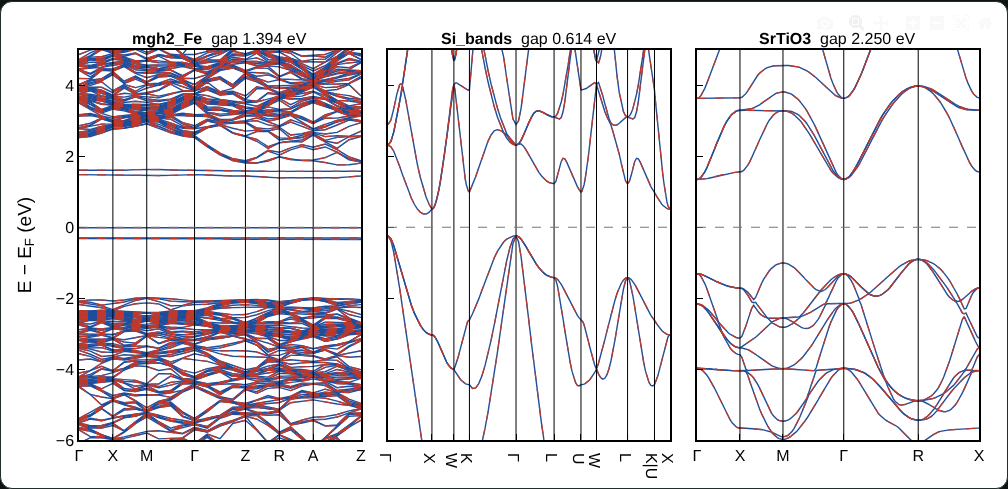
\includegraphics[width=\linewidth]{figures/comparison.png}
\end{tocentry}

\begin{abstract}
\BMR\ (Brillouin-zone Utilities for Materials Research) is a free, open-source toolkit that analyses the outputs of five electronic-structure packages (CASTEP, VASP, SIESTA, Quantum ESPRESSO and ORCA) through a single, code-agnostic data model. It computes spin-resolved band structures, total and projected densities of states, band edges and gaps by electron counting, effective masses and scissor or empirical band-gap corrections; it analyses point defects, polyhedral distortion and formation thermodynamics, and total, spin and difference charge densities with Voronoi and Bader partitions. Calculations from different codes can be compared side by side, the Fermi energy written by each code is never recomputed, and every session exports a BibTeX file with the methods actually used. The same analysis runs in a web browser without installation, in an offline desktop application and on high-performance computing clusters.
\end{abstract}

\section{Introduction}
First-principles post-processing is typically spread over several specialised tools tied to one code or one task, such as sumo\cite{ganose2018sumo} and pymatgen\cite{ong2013pymatgen} for band structures, VESTA\cite{momma2011vesta} for densities, the Bader program\cite{henkelman2006} for charges and cclib\cite{oboyle2008cclib} for quantum-chemistry outputs. Silent differences between them (energy references, density units, recomputed Fermi levels) are frequent sources of error, and results from different codes are rarely compared in one framework. \BMR\ unifies these analyses for plane-wave (CASTEP,\cite{clark2005castep} VASP,\cite{kresse1996vasp} Quantum ESPRESSO\cite{giannozzi2017}), localised-basis (SIESTA\cite{soler2002siesta}) and molecular (ORCA\cite{neese2020}) calculations.

\section{Implementation}
Code-specific readers convert every output to a common representation: eigenvalues in Hartree, reciprocal lattice in Bohr$^{-1}$, structures in \AA\ and densities in e\,\AA$^{-3}$. The analysis layer operates only on this representation and serves three front-ends with identical semantics: a single self-contained HTML application (JavaScript, Plotly.js) in which files are read locally and never uploaded; a desktop application that embeds the same interface offline through pywebview;\cite{pywebview} and a command-line program (one Python file depending only on numpy\cite{harris2020numpy} and matplotlib\cite{hunter2007matplotlib}) for batch use on clusters. Both implementations are cross-checked on the same inputs.

\section{Methods}
Densities of states are Gaussian-broadened sums, $g_s(E)=\sum_{\bm k}w_{\bm k}\sum_n\delta_\sigma(E-\varepsilon_{n\bm k s})$, and projections can be grouped by element, angular momentum, pseudopotential shell, magnetic component ($t_{2g}/e_g$) or atom. With $N_s$ electrons per spin, $E_g=\min_{\bm k}\varepsilon_{N_s+1,\bm k}-\max_{\bm k}\varepsilon_{N_s,\bm k}$ (the HOMO--LUMO gap for molecules). Effective masses follow from parabolic fits, $m^*/m_e=\hbar^2/(2m_e c_2)$. Because semilocal functionals underestimate gaps,\cite{perdew1983,sham1983} an optional scissor\cite{levine1989} shifts the unoccupied bands by $\Delta$, given directly, obtained from a reference gap, or estimated from the empirical relation $E_g^{G_0W_0}=1.358E_g^\mathrm{PBE}+0.904$\,eV;\cite{morales2017} the original gap is always reported. Defects are identified by minimum-image matching to a pure reference or by comparison with the supercell bulk, and characterised by Baur's index, quadratic elongation, angle variance\cite{robinson1971,baur1974} and effective coordination,\cite{hoppe1979} by the displacement field, and by formation energies $E_f=E_\mathrm{def}-E_\mathrm{pure}-\sum_in_i\mu_i$.\cite{freysoldt2014} The first Brillouin zone is built as the Wigner--Seitz cell of the reciprocal lattice on an LLL-reduced basis,\cite{lenstra1982} the lattice type is recognised from the shape of the zone, and high-symmetry points and paths follow Setyawan and Curtarolo,\cite{setyawan2010} with inputs written for CASTEP, VASP, Quantum ESPRESSO and SIESTA; space groups are determined with moyo,\cite{moyo} the successor of spglib,\cite{togo2024spglib} and structures can be read from CIF, POSCAR and other formats or from a library of 51 literature materials; all 14 Bravais lattices follow the Setyawan--Curtarolo convention, checked point by point against pymatgen. Charge densities support trilinear interpolation, Miller-plane slices, bond profiles, Voronoi\cite{voronoi1908,gellatly1982} and on-grid Bader\cite{henkelman2006} partitions, and density-difference descriptors (redistributed charge, dipole and radial accumulation).

\section{Validation}
Table~\ref{tab:v} lists results obtained with public outputs from the pymatgen, sisl, Quantum ESPRESSO and cclib test suites; Figure~\ref{fig:v} shows two examples.
\begin{table}\centering\small
\caption{Validation with real outputs (Kohn--Sham gaps of each functional).}\label{tab:v}
\begin{tabularx}{\linewidth}{@{}llX@{}}\toprule
Code & System & Result \\\midrule
CASTEP & MgH$_2$:Fe (162 atoms) & gap 1.394\,eV, indirect M$\to$R; Fe--H 1.65\,\AA\ ($-15.4$\% vs Mg--H) \\
VASP & Si (PBE) & gap 0.614\,eV, indirect; $m^*_e=0.94\,m_e$ (exp.\ 0.92) \\
VASP & Fe$_2$O$_3$ (LDA+U) & 20\,$\mu_\mathrm{B}$ (four high-spin Fe$^{3+}$) \\
SIESTA & SrTiO$_3$ (LDA) & gap 2.25\,eV, indirect R$\to\Gamma$; $\int\rho\,dV=40.000$\,e \\
SIESTA & Bi$_2$Se$_3$ (no spin--orbit) & gap 0.042\,eV, direct; eigenvalues identical to sisl \\
ORCA & divinylbenzene & HOMO--LUMO gap 5.18\,eV \\\bottomrule
\end{tabularx}
\end{table}
\begin{figure}\centering
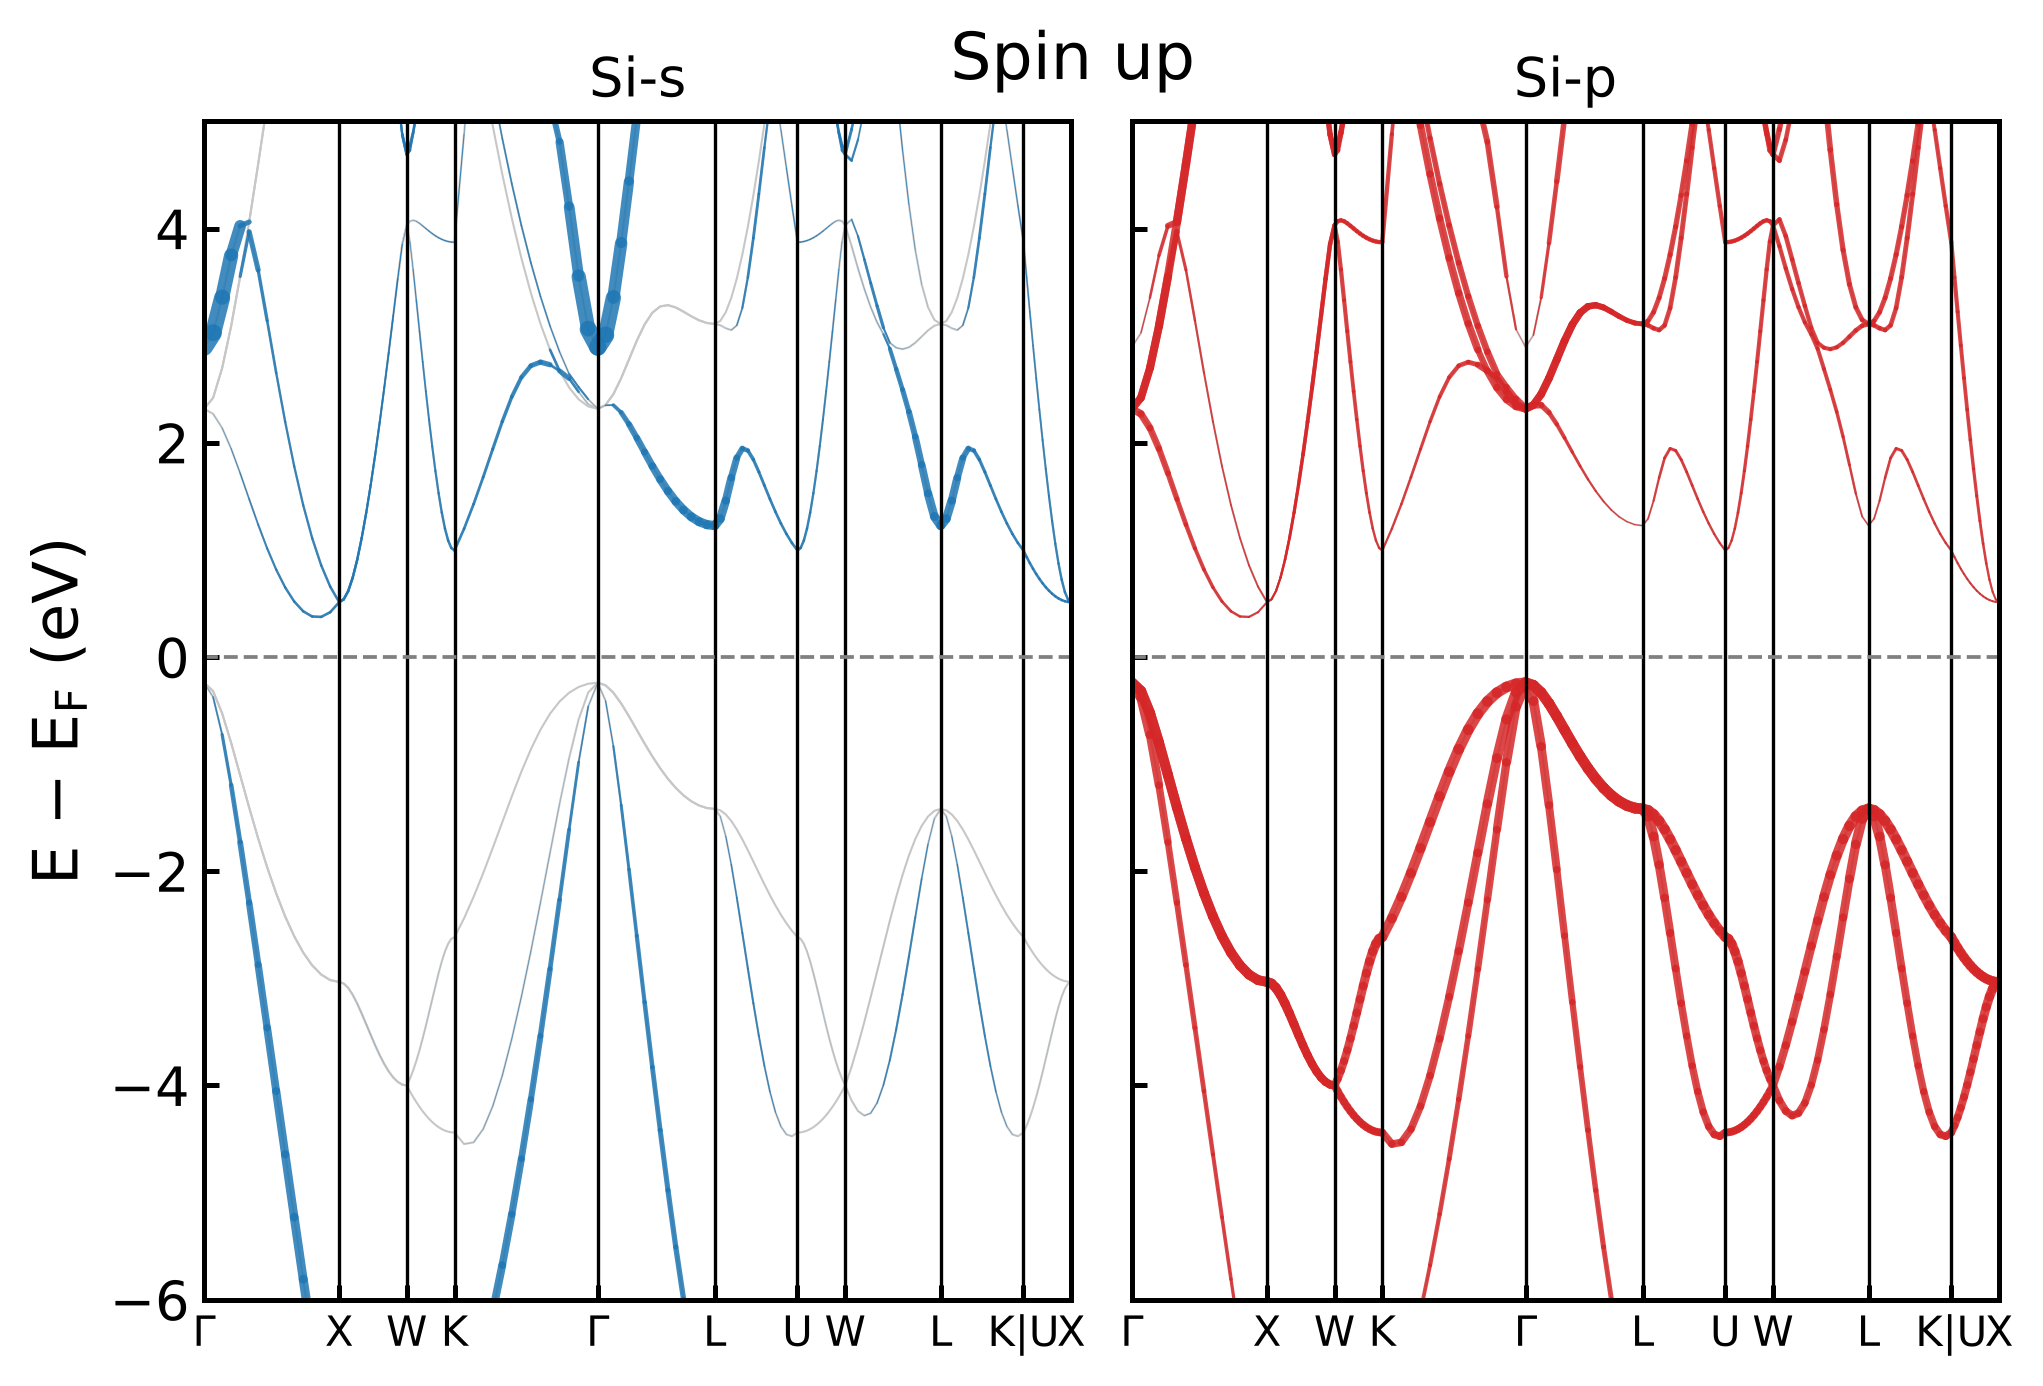
\includegraphics[width=0.48\linewidth]{figures/si_fat.png}\hfill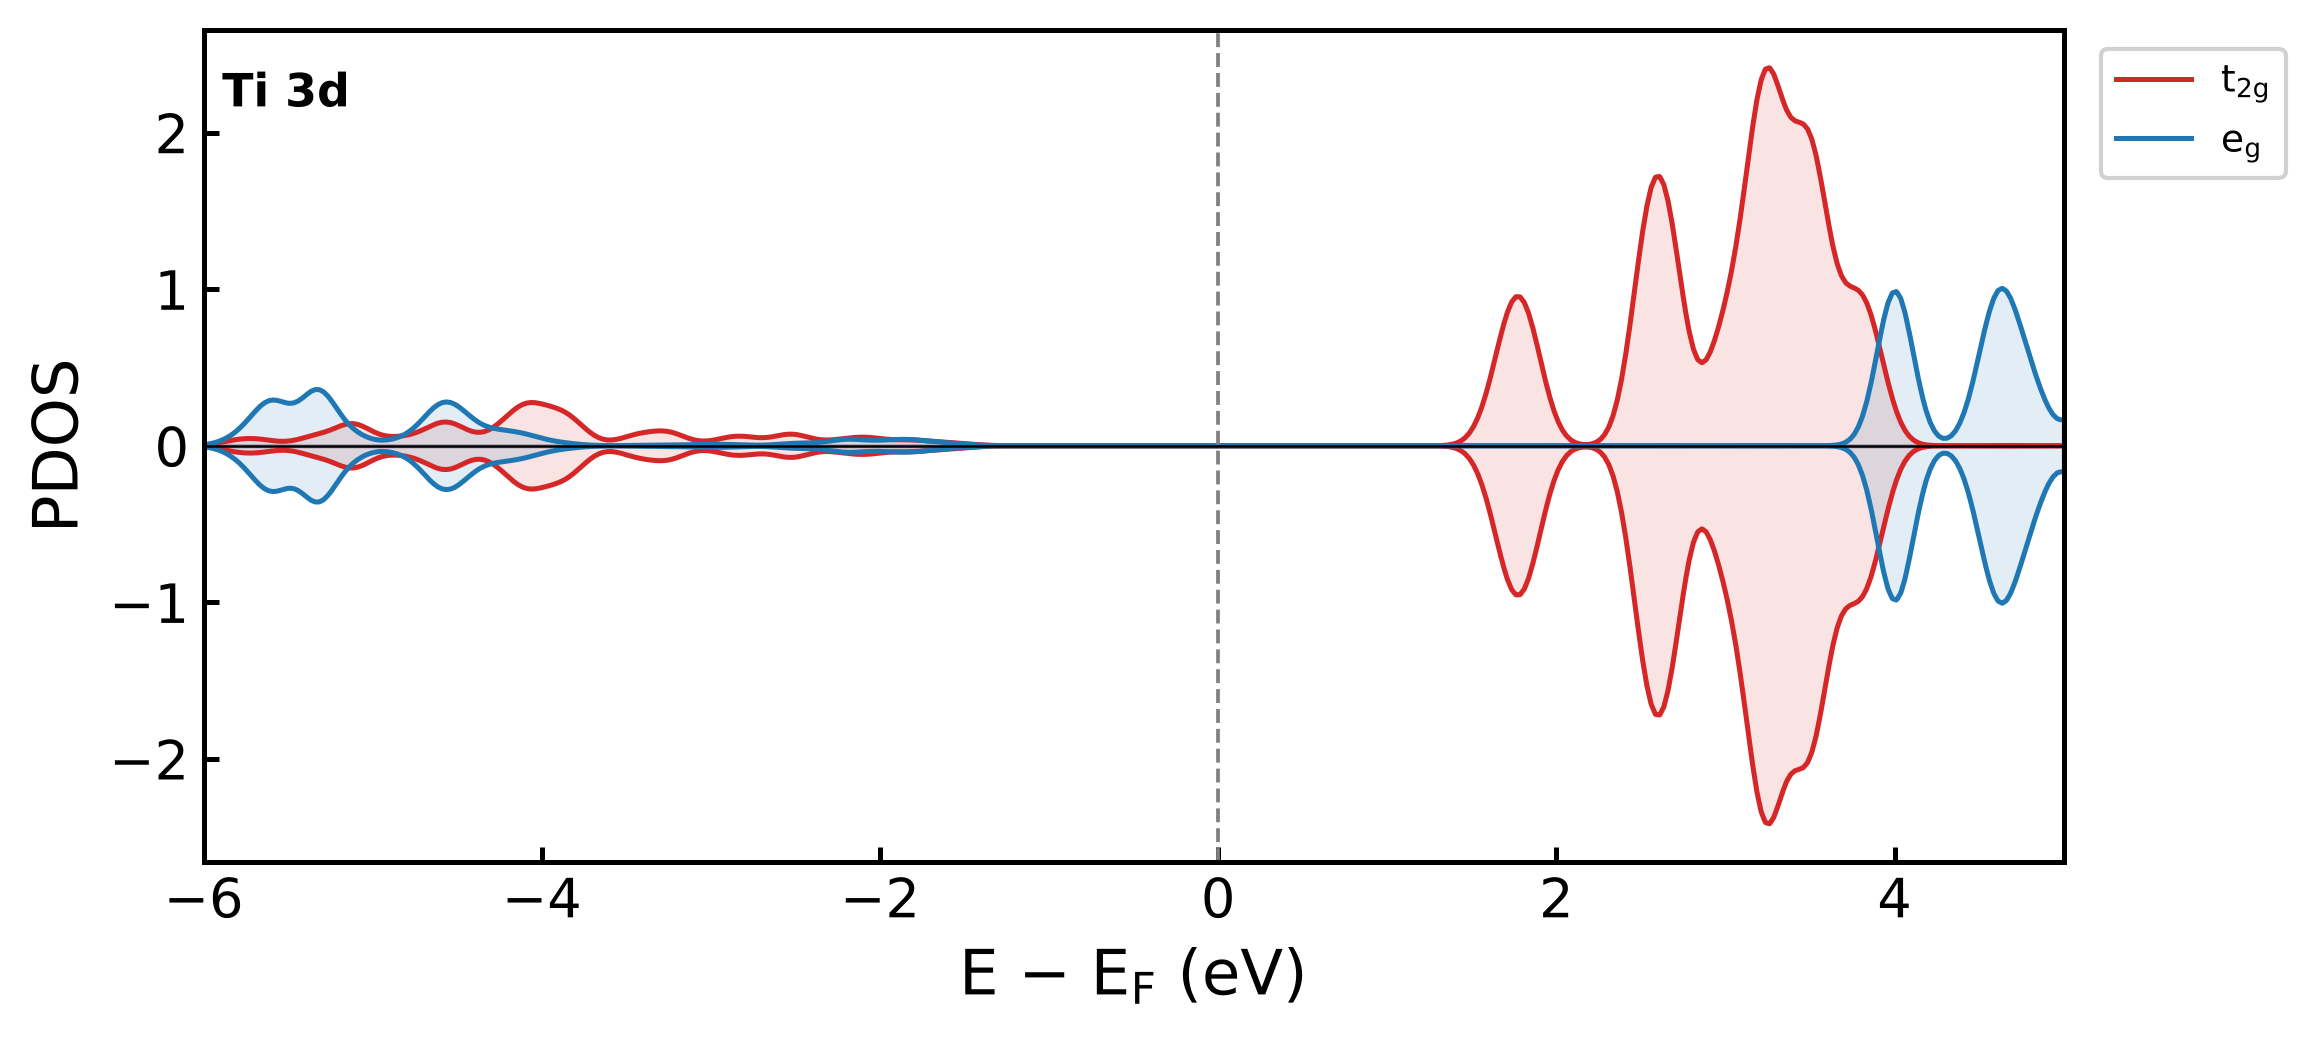
\includegraphics[width=0.48\linewidth]{figures/sto_t2g.png}
\caption{Projected bands of Si (VASP) and $t_{2g}/e_g$-resolved Ti 3d PDOS of SrTiO$_3$ (SIESTA).}\label{fig:v}
\end{figure}

On the same files, gaps, Fermi energies and orbital energies agree with pymatgen,\cite{ong2013pymatgen} sumo,\cite{ganose2018sumo} sisl and cclib\cite{oboyle2008cclib} to the printed precision, and refined Bader charges agree with pybader within 0.001\,e per atom. Electron counting avoids the spurious metallic classification produced by a 0.04\,meV numerical crossing of the CASTEP Fermi level in $E_\mathrm{F}$-based tools, and a fit with a linear term recovers the Si electron mass (0.94\,$m_e$; experiment 0.92\,$m_e$) where a parabola anchored at the sampled $\mathbf{k}$-point gives 0.68--1.54\,$m_e$. An automated test suite (80 tests) runs under continuous integration.

\section{Conclusions}
\BMR\ provides consistent, citable analyses of heterogeneous electronic-structure outputs in a browser, offline and on clusters, with the interface and tutorial available in six languages.

\section{Data and Software Availability}
Source code (GPL-3.0-or-later): \url{https://github.com/brunohdmacedo/brumare}; web application and tutorial: \url{https://brunohdmacedo.tech/brumare/}; Python package: \code{pip install brumare}. Version 1.3.0 should be archived with a DOI before submission. Validation inputs are public in the cited test suites; the MgH$_2$:Fe outputs are available from the author upon request.

\begin{acknowledgement}
The author thanks Benedet, R. O., without whom this work would never have happened; Prof. J. R. C. Salgado and Prof. R. S. da Lapa for supervision; and CNPq (Brazil) for a master's scholarship. Generative AI (Anthropic's Claude) was used extensively to help write and refactor parts of the source code, translate the interface and tutorial, draft documentation, and draft and edit this manuscript; all AI-assisted code was reviewed and verified by the author against real outputs of the five supported codes and by cross-checking the two implementations, and the author takes full responsibility for the content.
\end{acknowledgement}

\bibliography{references}
\end{document}
